\begin{frame}
  \begin{center}
    \large{1. Noyaux}
  \end{center}
\end{frame}

\begin{frame}
  \frametitle{1.1 Produit scalaire}
  \begin{itemize}
  \item $\langle \xvec, \xvec^\prime \rangle = \sum_{j=1}^p x_j x_j^\prime$
  \item $\langle \xvec, \xvec^\prime \rangle = \ltwonorm{\xvec} \ltwonorm{\xvec^\prime} \cos \theta$ \hspace{1em}
     $\ltwonorm{\xvec}^2 = \langle \xvec, \xvec \rangle$
  \item Interprétable comme \blue{mesure de similarité}
  \item \blue{Forme définie positive bilinéaire :}
    \begin{itemize}
    \item $\langle \xvec, \xvec^\prime \rangle = \langle \xvec^\prime, \xvec \rangle$
      pour tout $\xvec, \xvec^\prime \in \mathcal{X}$
    \item $\langle \xvec + \zvec, \xvec^\prime \rangle = \langle \xvec, \xvec^\prime \rangle +
      \langle \zvec, \xvec^\prime \rangle$       pour tout $\xvec, \xvec^\prime, \zvec \in \mathcal{X}$
    \item $\langle a \xvec, \xvec^\prime \rangle = a \langle \xvec, \xvec^\prime \rangle$ pour tout $a \in \RR$
    \item $\langle \xvec, \xvec \rangle \geq 0$ et $\langle \xvec, \xvec \rangle = 0 \text{ ssi } \xvec = 0$
    \end{itemize}
  \item Apparaît dans de nombreux algorithmes d'apprentissage.
  \end{itemize}
\end{frame}

\begin{frame}
  \frametitle{1.2 Noyau}
  \begin{itemize}
  \item \blue{Généralisation} du produit scalaire : $k: \xcal \times \xcal \rightarrow \RR$
    \begin{itemize}
    \item \blue{sémantiquement} une similarité
    \item \blue{mathématiquement} une forme définie positive 
    \end{itemize}
  \item Aronszajn: Si $k$ est semi-définie positive\footnote{Pour tout
      $m \in \NN^*$, pour tout
      $\{\xvec_1, \xvec_2, \dots, \xvec_m\} \in \xcal,$ la matrice
      $K \in \RR^{m \times m}$ telle que $K_{il} = k(\xvec_i, \xvec_l)$ est
      semi-définie positive}, il existe un espace de Hilbert $\hcal$ et une application
    $\varphi: \xcal \rightarrow \hcal$ telle que
    $\textcolor{MyOrange}{k(\xvec, \xvec^\prime) = \langle \varphi(\xvec), \varphi(\xvec^\prime)\rangle_{\hcal}}$
    pour tout $\xvec, \xvec^\prime, \zvec \in \mathcal{X}$
  \end{itemize}
\end{frame}

\begin{frame}
  \frametitle{1.3 Astuce du noyau}
  \begin{itemize}
    \item[]    $\textcolor{MyOrange}{k(\xvec, \xvec^\prime) = \langle \varphi(\xvec), \varphi(\xvec^\prime)\rangle_{\hcal}}$
    \item Si un algorithme ne fait intervenir les éléments de $\xcal$ que dans
      des produits scalaires, \blue{remplacer ces produits scalaires} par $k$ est
      équivalent à appliquer l'algorithme dans $\hcal$ après avoir appliqué
      $\varphi$
    \item Utile \blue{si $k$ est plus simple à calculer que $\varphi$}
      \pause
    \item Exemple : \blue{noyau quadratique}
      $k: (\xvec, \xvec^\prime) \mapsto (1 + \langle \xvec, \xvec^\prime \rangle)^2$
    \item[] Équivaut à $\varphi : (x_1, x_2, \dots, x_p) \mapsto (1, x_1, \dots, x_p,
      x_1^2, x_2^2, \dots, x_p^2, \sqrt{2} x_1 x_2, \dots, \sqrt{2}x_{p-1}x_p).$
  \end{itemize}
\end{frame}

\begin{frame}
  \frametitle{Noyau quadratique}
  \begin{itemize}
  \item[] $k: (\xvec, \xvec^\prime) \mapsto (1 + \langle \xvec, \xvec^\prime \rangle)^2$
  \item[] Équivaut à $\varphi : (x_1, x_2, \dots, x_p) \mapsto (1, x_1, \dots, x_p,
    x_1^2, x_2^2, \dots, x_p^2, \sqrt{2} x_1 x_2, \dots, \sqrt{2}x_{p-1}x_p).$
  \end{itemize}
  \begin{center}
    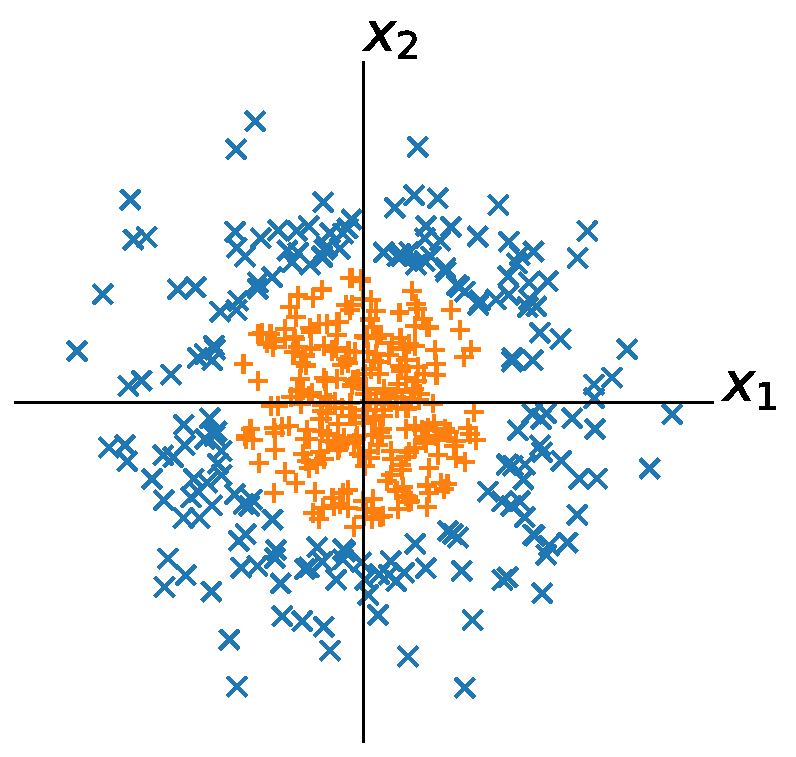
\includegraphics[width=0.4\textwidth]{figures/circular-separable}%
    \hfill
    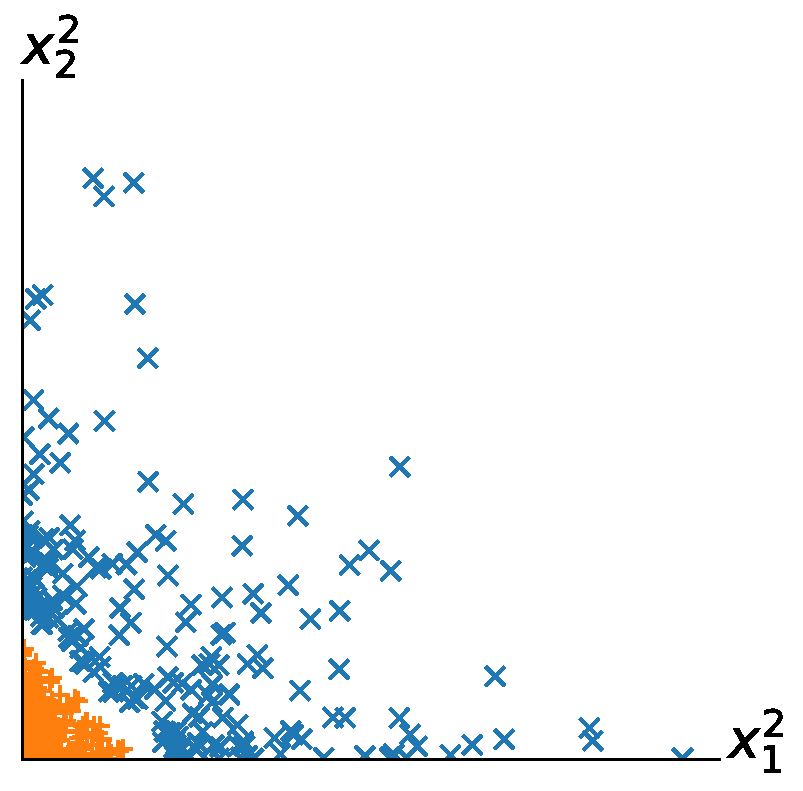
\includegraphics[width=0.4\textwidth]{figures/circular-separable-mapped}%
  \end{center}
\end{frame}

\begin{frame}
  \frametitle{1.4 Régression ridge à noyau}
  \begin{itemize}
  \item \blue{Régression ridge :}
    {\footnotesize $\argmin_{\betavec \in \RR^{p+1}} \frac1n \left(\yvec - X \betavec \right)^\top
      \left(\yvec - X \betavec \right) + \lambda \ltwonorm{\betavec} $}      
    \begin{itemize}
    \item Solution : $\betavec^* = \left(X^\top X + \lambda I_p \right)^{-1} X^\top \yvec$
    \item Modèle : $f: \xvec \mapsto \langle \betavec^*, \xvec \rangle$
    \end{itemize}
  \item Reformulation :
    $f: \xvec \mapsto \textcolor{Aubergine}{\xvec X^\top} \left( \lambda I_n +
      \textcolor{MyPink}{XX^\top} \right)^{-1} \yvec $
    \pause
    \begin{itemize}
    \item $\textcolor{Aubergine}{\xvec X^\top} \in \RR^n$ a pour $i$-ème entrée :
      $\textcolor{Aubergine}{\langle \xvec, \xvec_i \rangle}$    
    \item $\textcolor{MyPink}{X X^\top} \in \RR^{n \times n}$ a pour entrée $(i,l)$ :
      $\textcolor{MyPink}{\langle \xvec_i, \xvec_l \rangle}$
    \end{itemize}
    \pause
  \item \blue{Kernelization :} remplacer $\textcolor{Aubergine}{\xvec X^\top}$ par
    $\textcolor{Aubergine}{\kappa} \in \RR^n$ tel que
    $\textcolor{Aubergine}{\kappa_i = k(\xvec, \xvec_i)}$ et $\textcolor{MyPink}{XX^\top}$ par
    $\textcolor{MyPink}{K} \in \RR^{n \times n}$ telle que $\textcolor{MyPink}{K_{il} = k(\xvec_i, \xvec_l)}$
  \item[] équivaut à transformer les données par $\varphi$ puis apprendre une régression ridge, \blue{pour environ le même coût algorithmique}
  \end{itemize}
\end{frame}

\begin{frame}
  \frametitle{1.5 Exemples de noyaux}
  \begin{itemize}
  \item \blue{Noyau quadratique} $k: (\xvec, \xvec^\prime) \mapsto (1 + \langle \xvec, \xvec^\prime \rangle)^2$
  \item[] $\varphi$ calcule tous les monômes de degré au plus 2 de $x_1, x_2, \dots, x_p$ 
    \pause
  \item \blue{Noyau polynomial} $k: (\xvec, \xvec^\prime) \mapsto (1 + \langle \xvec, \xvec^\prime \rangle)^d$
  \item[] $\varphi$ calcule tous les monômes de degré au plus $d$ de $x_1, x_2, \dots, x_p$ 
    \pause 
  \item \blue{Noyau RBF gaussien} $k: (\xvec, \xvec^\prime) \mapsto
    \exp\left( - \frac{\ltwonorm{\xvec - \xvec^\prime}^2}{\sigma^2} \right)$
  \item[] $\varphi$ calcule tous les monômes de $x_1, x_2, \dots, x_p$ 
  et $\hcal$ est de dimension infinie. 
  \end{itemize}
\end{frame}

\begin{frame}
  \frametitle{1.5 Exemples de noyaux}
  \begin{itemize}
  \item \blue{Noyau pour chaîne de caractères} $k: (\xvec, \xvec^\prime) \mapsto
    \sum_{u \in \aset^m} \psi_u(\xvec) \psi_u(\xvec^\prime)$
    \begin{itemize}
    \item $\aset^m$ = l'ensemble des chaînes de $m$ caractères sur l'alphabet $\aset$
    \item $\psi_u(\xvec) = 1$ si $u$ est une sous-chaîne de $\xvec$ et $0$ sinon.
    \end{itemize}
  \pause
  \item $k(\xvec, \xvec^\prime)$ est le nombre de chaînes de $m$ caractères
    communes à $\xvec$ et $\xvec^\prime$ et peut être calculé en
    $\mathcal{O}(|\xvec|)$ au lieu de $\mathcal{O}(|\aset|^m)$.
    \pause
  \item Si $m=8$, $|\aset|=20$ et en moyenne $|\xvec| = 485,$ on compare 25,6 milliards
    d'opérations à moins de 500.
  \end{itemize}
\end{frame}

\begin{frame}
  \frametitle{Recap : Méthodes à noyau}
  \begin{itemize}
  \item \black{Idée :} Remplacer dans un algorithme tous les \blue{produits scalaires} par des \blue{noyaux}
  \item Apprendre des modèles \blue{non-linéaires} efficacement
  \item Appliquer des modèles linéaires à des \blue{objets} dont la représentation en $p$ dimensions n'est pas évidente (images, protéines, graphes, etc.)
    
  \end{itemize}
\end{frame}

\begin{frame}
  \begin{center}
    \large{2. Machines à vecteurs de support}
  \end{center}
\end{frame}

\begin{frame}[t]
  \frametitle{2.1 Formulation primale}
  \begin{itemize}
  \item Classification binaire, $\ycal = \{-1, 1\}$ 
    \[\argmin_{\betavec \in \RR^p, b \in \RR} \frac12 \ltwonorm{\betavec}^* + C \sum_{i=1}^n
      \max\left( 0, 1 - y_i \left( \langle \betavec, \xvec_i \rangle + b \right)\right)\]
  \end{itemize}
  \begin{center}
    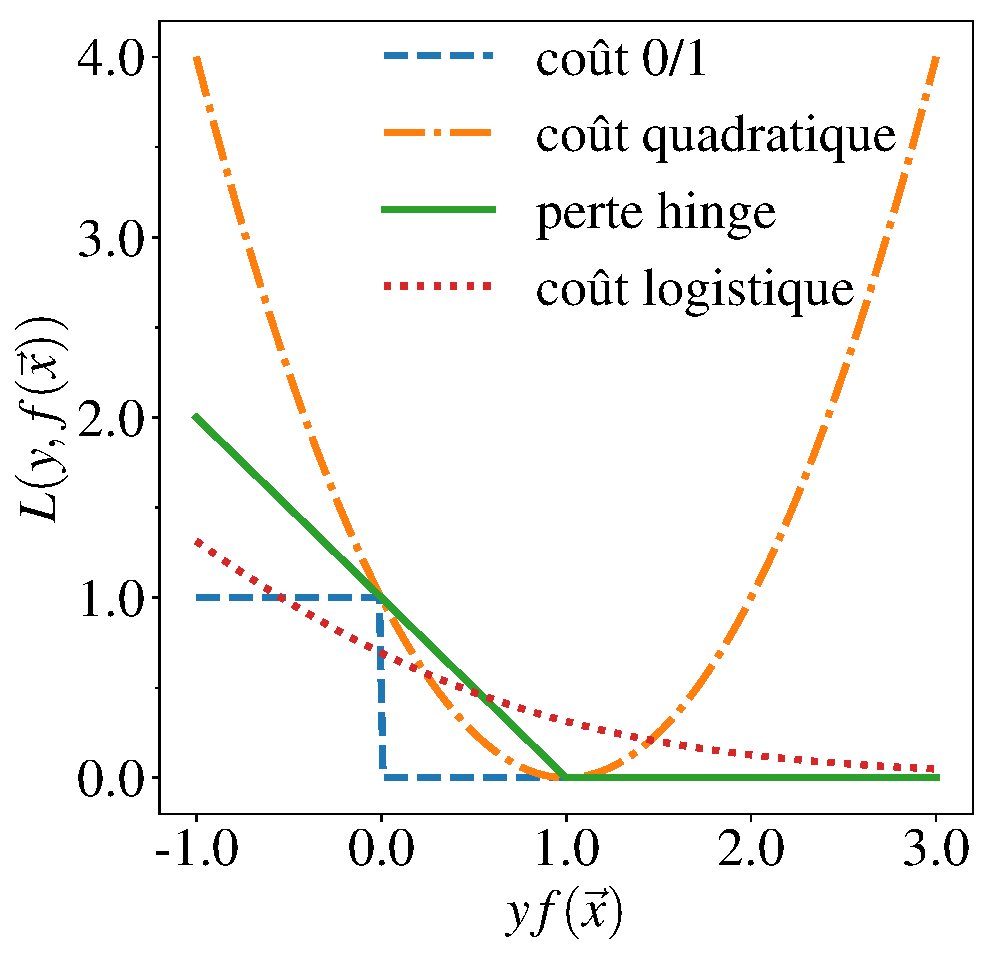
\includegraphics[width=0.5\textwidth]{figures/classif_losses}%
  \end{center}
\end{frame}

\begin{frame}[t]
  \frametitle{2.1 Formulation primale}
  \begin{itemize}
  \item Classification binaire, $\ycal = \{-1, 1\}$ 
    \[\argmin_{\betavec \in \RR^p, b \in \RR} \frac12 \ltwonorm{\betavec}^* + C \sum_{i=1}^n
      \max\left( 0, 1 - y_i \left( \langle \betavec, \xvec_i \rangle + b \right)\right)\]
  \end{itemize}
  \begin{center}
    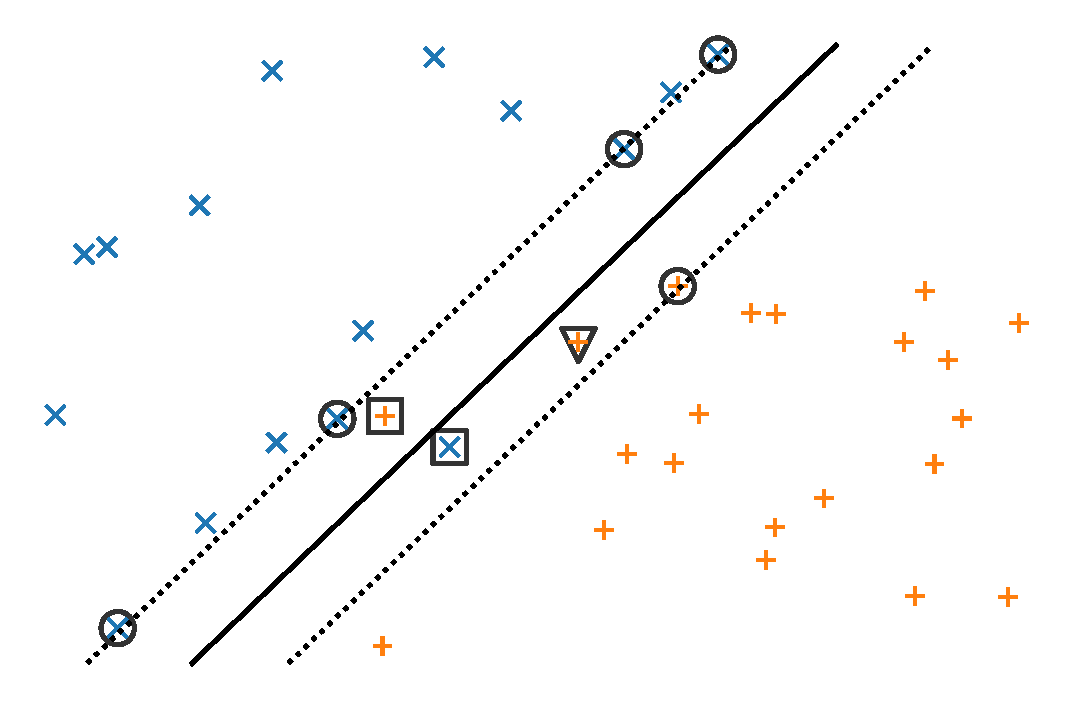
\includegraphics[width=0.7\textwidth]{figures/non-linearly-separable}%
  \end{center}
\end{frame}

\begin{frame}[t]
  \frametitle{2.2 Formulation duale}
    {\small \[\argmax_{\alphavec \in \RR^n} \sum_{i=1}^n \alpha_i - \frac12 \sum_{i=1}^n \sum_{l=1}^n
      \alpha_i \alpha_l y_i y_l \langle \xvec_i, \xvec_l \rangle   \]}
  \begin{itemize}
  \item[] sous les contraintes $\sum_{i=1}^n \alpha_i y_i = 0$  et $0 \leq \alpha_i \leq C$ 
  \item Modèle : $f: \xvec \mapsto \sum_{i=1}^n \alpha_i y_i \langle \xvec_i, \xvec \rangle$
  \end{itemize}
\end{frame}

\begin{frame}[t]
  \frametitle{2.3 SVR (Support Vector Regression)}
  \begin{itemize}
  \item Perte $\varepsilon$-insensible :
    \[L(y, f(\xvec) = \max(0, |f(\xvec) - y| - \varepsilon)\]
  \end{itemize}
  \begin{center}
    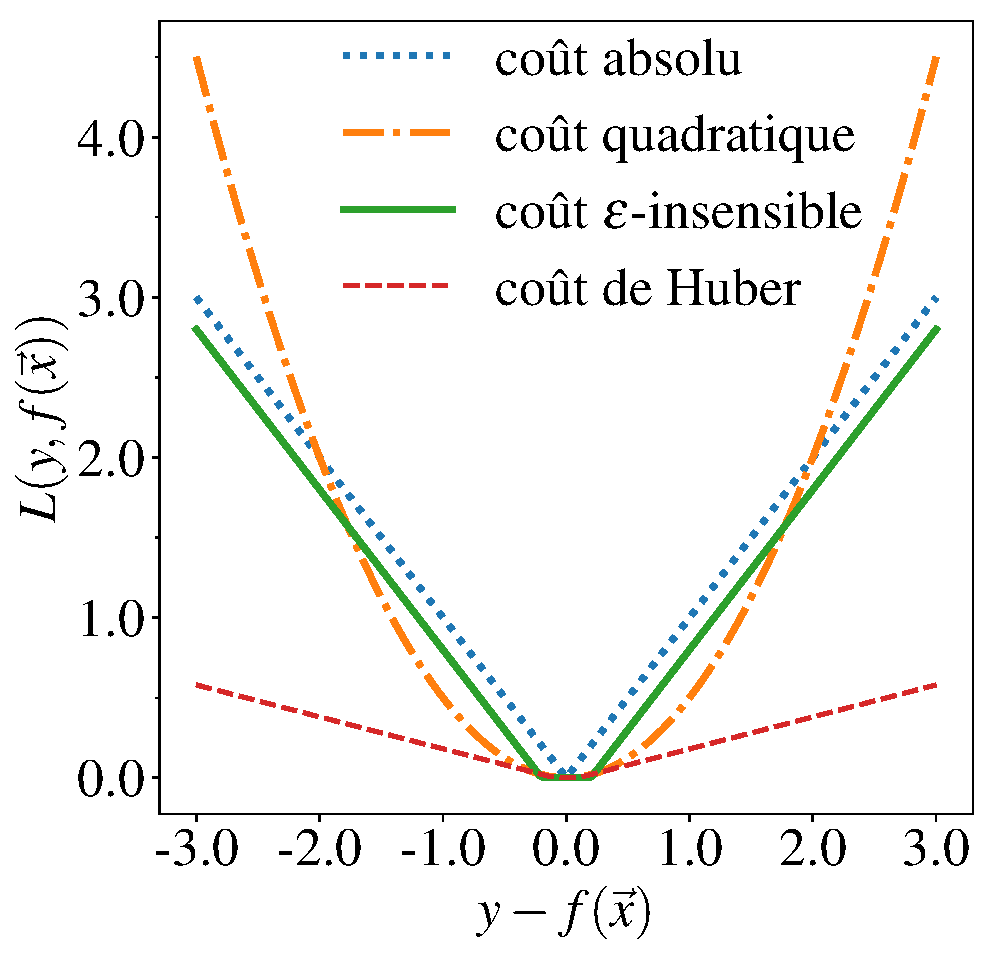
\includegraphics[width=0.5\textwidth]{figures/regression_losses}%
  \end{center}
\end{frame}
